\chapter{Implementation}

% ----------------------------------------------------------------------------- Diagrames-UML

\section{Diagramme r\'etrog\'en\'er\'es de packages et de classes}

\begin{figure}[h]
    \centering
    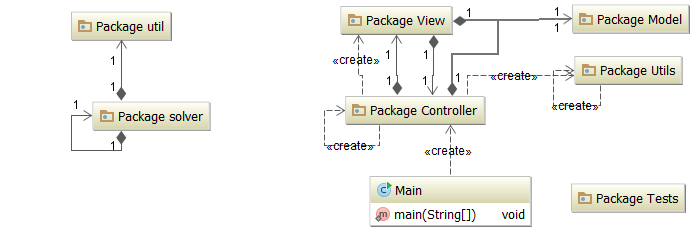
\includegraphics[width=150mm]{../diagrams/classes_packages/final_classes_packages/packages.png}
    \caption{Diagramme r\'etrog\'en\'er\'e UML de package principale}
    \label{diagram:gen_uml_global}
\end{figure}
\pagebreak

\subsection{Utilitaires (Utils)}

\begin{figure}[h]
    \centering
    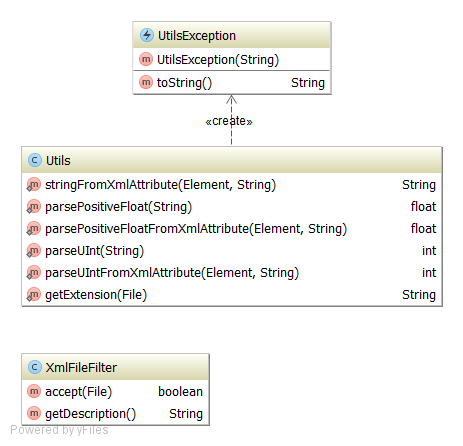
\includegraphics[width=100mm]{../diagrams/classes_packages/final_classes_packages/utils/package_utils.png}
    \caption{Diagramme r\'etrog\'en\'er\'e UML du package Utils}
    \label{diagram:gen_uml_utils}
\end{figure}
\pagebreak

\subsection{Mod\`ele (Model)}

\begin{figure}[h]
    \centering
    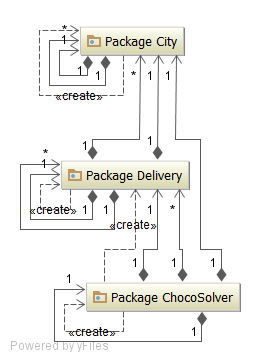
\includegraphics[width=80mm]{../diagrams/classes_packages/final_classes_packages/model/package_model.png}
    \caption{Diagramme r\'etrog\'en\'er\'e UML du package Model}
    \label{diagram:gen_uml_model}
\end{figure}
\pagebreak

\subsubsection{Mod\`ele Ville (Model.City)}

\begin{figure}[h]
    \centering
    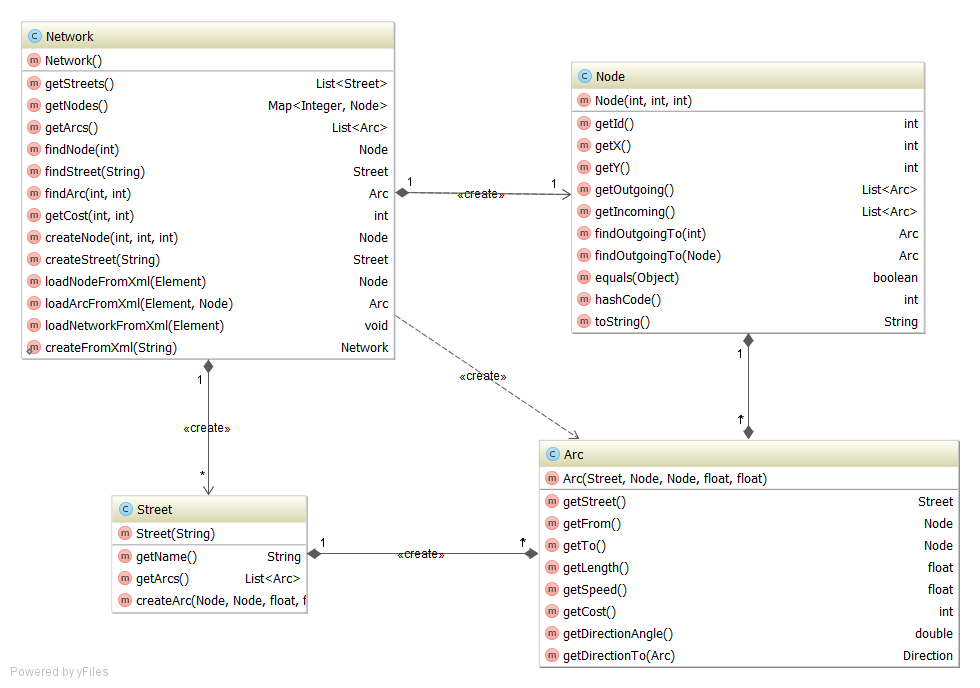
\includegraphics[width=160mm]{../diagrams/classes_packages/final_classes_packages/model/city.png}
    \caption{Diagramme r\'etrog\'en\'er\'e UML du package Model.City}
    \label{diagram:gen_uml_model_city}
\end{figure}
\pagebreak

\subsubsection{Mod\`ele Livraison (Model.Delivery)}

\begin{figure}[h]
    \centering
    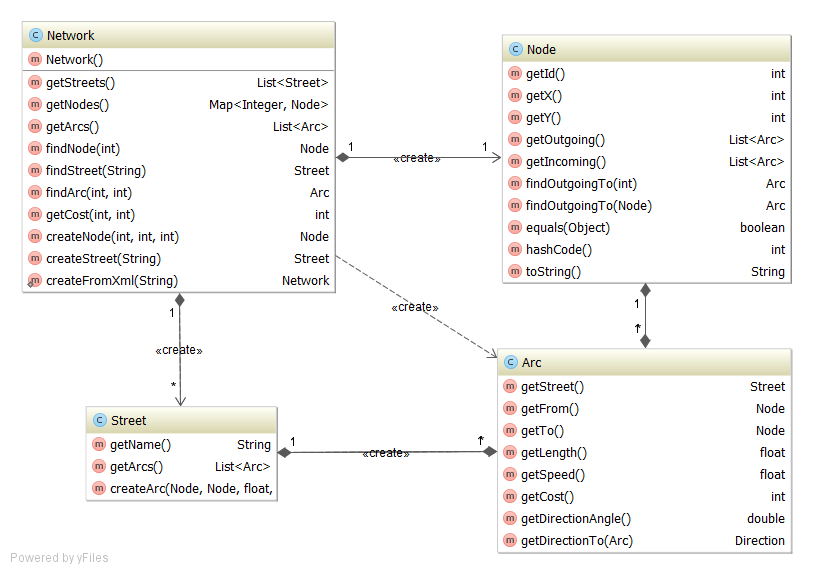
\includegraphics[width=160mm]{../diagrams/classes_packages/final_classes_packages/model/delivery.png}
    \caption{Diagramme r\'etrog\'en\'er\'e UML du package Model.Delivery}
    \label{diagram:gen_uml_model_delivery}
\end{figure}
\pagebreak

\begin{landscape}
\subsubsection{Mod\`ele Resolution Choco (Model.ChocoSolver)}

\begin{figure}[h]
    \centering
    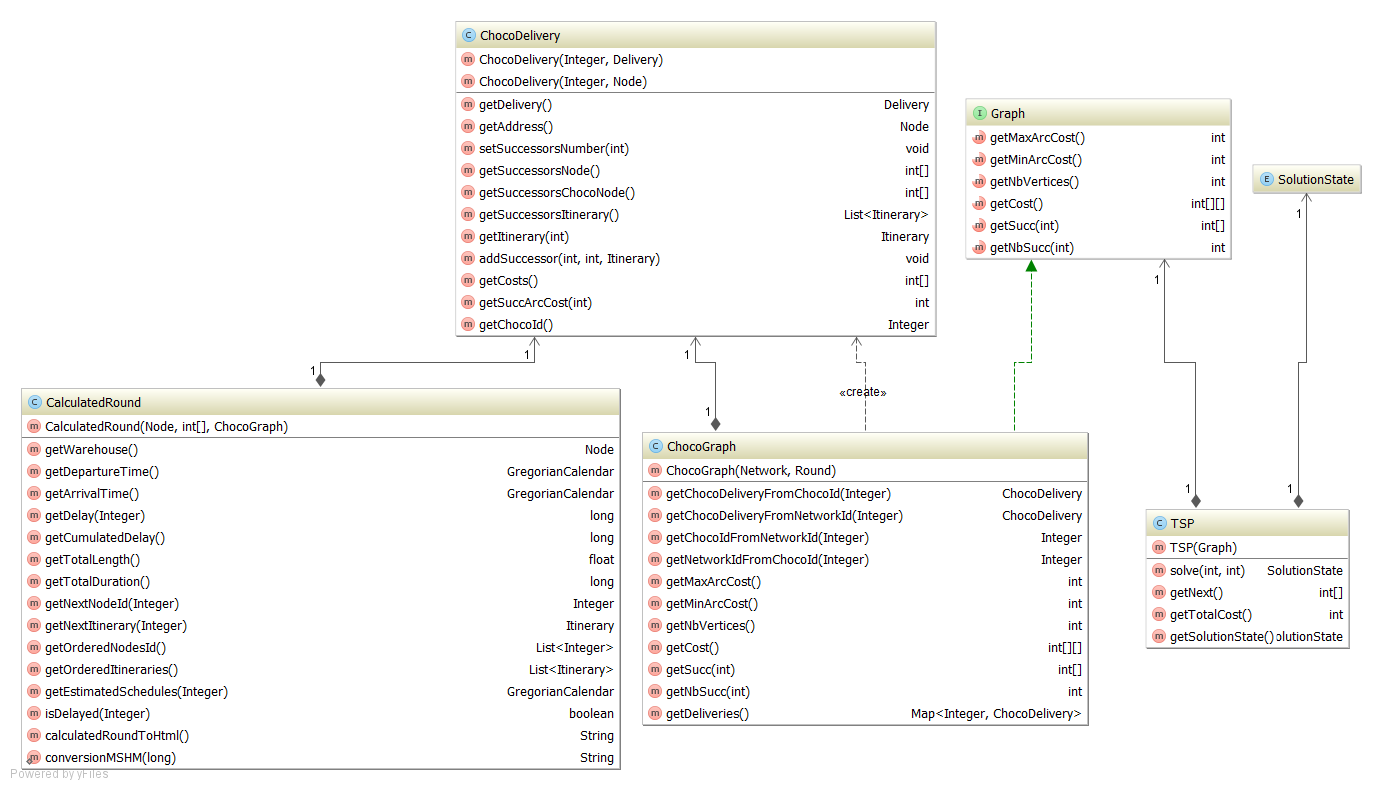
\includegraphics[width=200mm]{../diagrams/classes_packages/final_classes_packages/model/chocoSolver.png}
    \caption{Diagramme r\'etrog\'en\'er\'e UML du package Model.ChocoSolver}
    \label{diagram:gen_uml_model_choco}
\end{figure}
\end{landscape}
\pagebreak

\subsection{Vue (View)}

\begin{figure}[h]
    \centering
    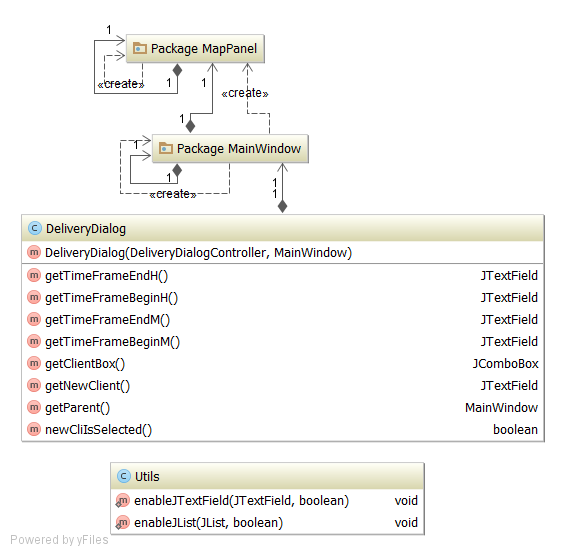
\includegraphics[width=120mm]{../diagrams/classes_packages/final_classes_packages/view/view.png}
    \caption{Diagramme r\'etrog\'en\'er\'e UML du package View}
    \label{diagram:gen_uml_view}
\end{figure}
\pagebreak

\subsubsection{Vue Carte (View.MapPanel)}

\begin{figure}[h]
    \centering
    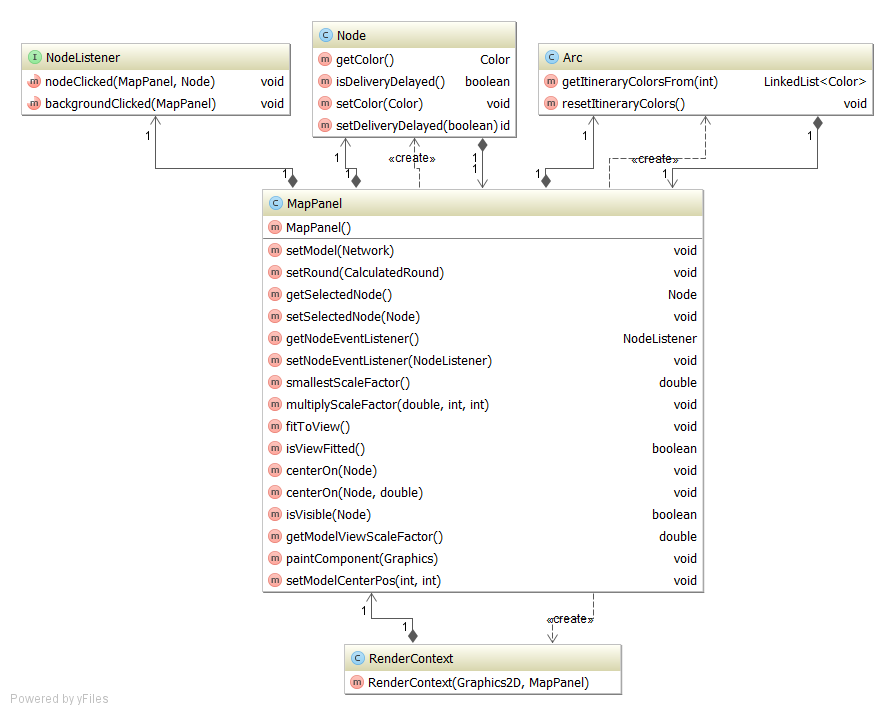
\includegraphics[width=160mm]{../diagrams/classes_packages/final_classes_packages/view/package_map.png}
    \caption{Diagramme r\'etrog\'en\'er\'e UML du package View.MapPanel}
    \label{diagram:gen_uml_view_map}
\end{figure}
\pagebreak

\subsection{Controlleur (Controller)}

\begin{figure}[h]
    \centering
    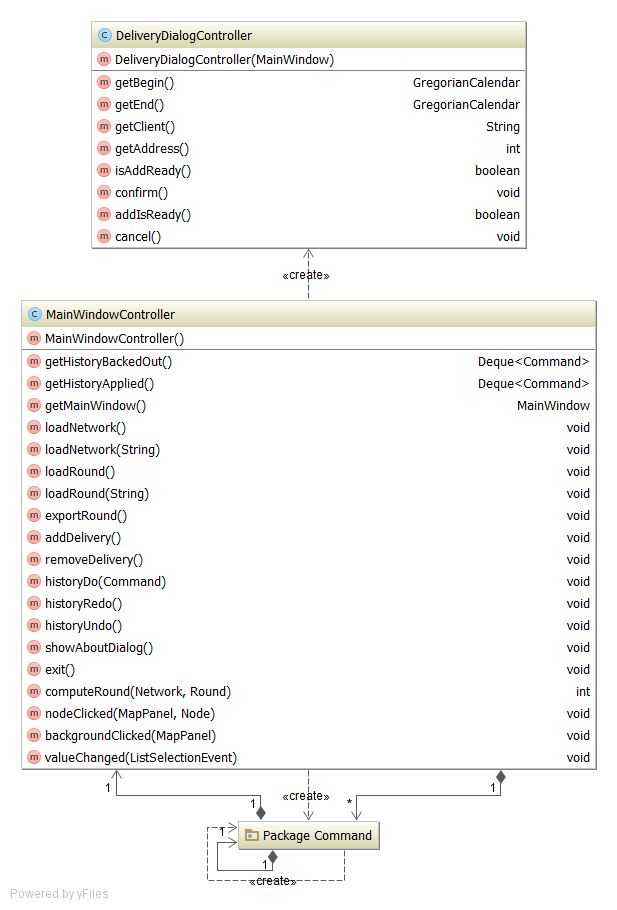
\includegraphics[width=100mm]{../diagrams/classes_packages/final_classes_packages/controller/controller.png}
    \caption{Diagramme r\'etrog\'en\'er\'e UML du package Controller}
    \label{diagram:gen_uml_controller}
\end{figure}
\pagebreak

\begin{landscape}
\subsubsection{Commande (Controller.Command)}

\begin{figure}[h]
    \centering
    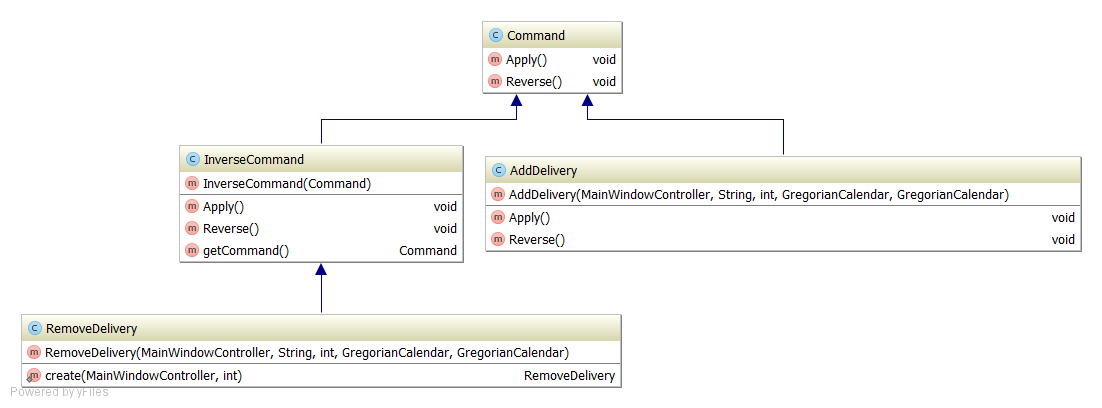
\includegraphics[width=240mm]{../diagrams/classes_packages/final_classes_packages/controller/package_command.png}
    \caption{Diagramme r\'etrog\'en\'er\'e UML du package Controller.Command}
    \label{diagram:gen_uml_controller_command}
\end{figure}
\end{landscape}

